\section{Introduction}
\label{sec: introduction}

\IEEEPARstart{W}{ith} the great success of deep learning in computer vision, this decade has witnessed an explosion of deep learning-based computer vision-based applications. Because of the huge computational resource consumption for deep learning applications (e.g., inferring an image on VGG19~\cite{VGG19} requires $20$ GFLOPs of GPU resource), in today's online computer vision-based applications, users usually have to upload the input images to the central cloud service providers (e.g., SenseTime, Baidu Vision and Google Vision, etc.), leading to a significant upload traffic load. 

To reduce the upload traffic load, it is straightforward that an image should be compressed before one uploads it. Though JPEG has been used as the \emph{de facto} image compression and encapsulation method, its performance for the deep computer vision models is not satisfactory. Liu et al.~\cite{DeepN-JPEG} showed that by re-designing the quantization table in the default JPEG configuration, one can compress an image to a smaller version while maintaining the same inference accuracy for a deep computer vision model. However, such quantization solutions usually assume the inference model is fixed. 

We then raise an intuitive question: to make it practically useful, can we select the JPEG configuration adaptively for different online computer vision-based services, without any prior knowledge of the original model and input images? In this paper, we propose a reinforcement learning-based framework to select JPEG configurations adaptively. In our solution, we tackle the following design challenges.

\begin{itemize}

\item \emph{Lack of information about the cloud-based computer vision models.} Previous studies~\cite{DeepN-JPEG, torfason2018towards, gueguen2018faster}, generally assume that the details of the computer vision models are available so that they can adjust the JPEG configuration according to the model structure, e.g., one can train a model to determine the JPEG configuration by plugging the original computer vision model into it. However, the structure details of online computer vision models are usually proprietary and not open to the users. 

\item \emph{Different cloud-based computer vision models need different JPEG configurations.} As an adaptive JPEG configuration solution, we target to provide a solution that is adaptive to different online computer vision-based services, i.e., it can \emph{generate} JPEG configuration for different models. However, today's cloud-based computer vision algorithms, based on deep and convolutional computations, are quite hard to understand. The same compression quality level could lead to a totally different accuracy performance. Some examples are shown in Figure~\ref{fig: compress_accuracy}: picture 1a and 1b, 2a and 2b are visually similar for human beings, but the deep learning model gives different inference results, only because they are compressed at different quality levels. And such a relationship is not apparent, e.g., picture 3b is highly compressed and looks destroyed comparing to picture 3a, but the deep learning model can still recognize it. This phenomenon is also presented in~\cite{delac2005effects} and commonly seen in adversarial neural network researches~\cite{yuan2019adversarial, evtimov2018robust}.

\item \emph{Lack of well-labeled training data.} In our problem, one is not provided the well-labeled data on which image should be compressed to which quality level, as in conventional supervised deep learning tasks. In practice, such an image compression module is usually utilized in an online manner, and the solution has to learn from the images it uploads automatically. 
\end{itemize} 

\begin{figure*}[htbp]
%	\begin{tabular}{cc}
	\begin{minipage}{0.5\linewidth}
		\centerline{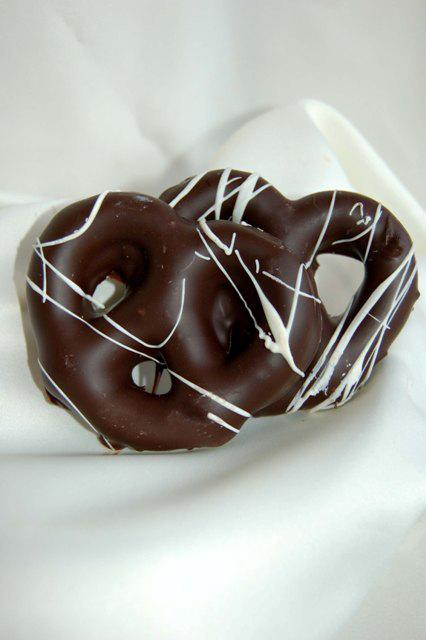
\includegraphics[width=6.0cm, trim=0 150 0 150, clip]{figures/donut_q75.jpeg}}
		\centerline{(1a) Q=75}
%		\centerline{Face++ prediction=["donut"]}
		\centerline{Face++ prediction \ = \ ["donut"]}
		\vspace{0.4cm}
	\end{minipage}
	\hfill
	\begin{minipage}{0.5\linewidth}
		\centerline{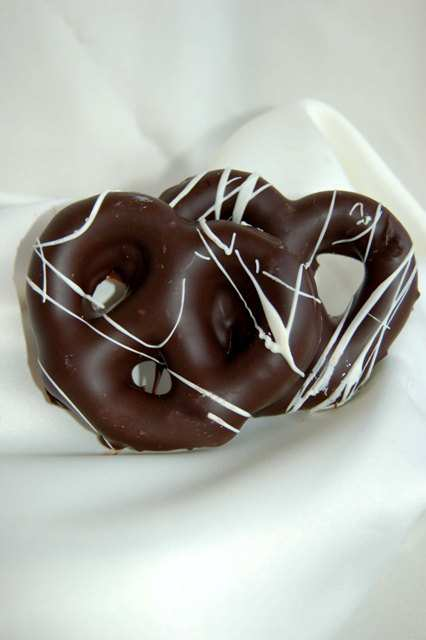
\includegraphics[width=6.0cm, trim=0 150 0 150, clip]{figures/donut_q55.jpeg}}
		\centerline{(1b) Q=55}
%		\centerline{Face++ prediction=[]}
		\centerline{Face++ prediction \ = \ ["biscuit"]}
		\vspace{0.4cm}
	\end{minipage}
	\vfill	
	\begin{minipage}{0.5\linewidth}
		\centerline{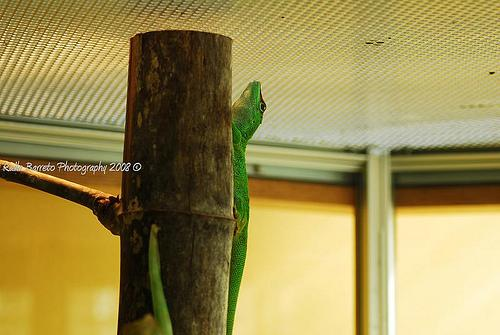
\includegraphics[width=6.0cm, trim=0 0 0 0]{figures/chameleon_q75.jpeg}}
		\centerline{(2a) Q=75}
% 		\centerline{\quad Baidu prediction=["chameleon"]}
		\centerline{Baidu prediction \ = \ ["chameleon"]}
		\vspace{0.4cm}
	\end{minipage}
	\hfill
	\begin{minipage}{0.5\linewidth}
		\centerline{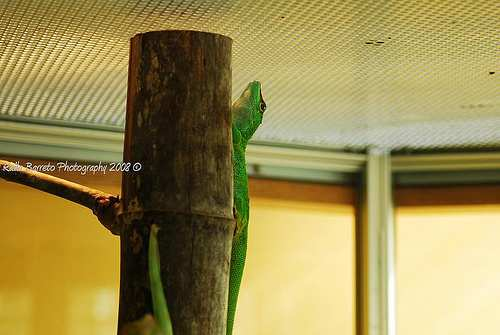
\includegraphics[width=6.0cm, trim=0 0 0 0]{figures/chameleon_q55.jpeg}}
		\centerline{(2b) Q=55}
% 		\centerline{\qquad Baidu prediction=["electric fan"]}
 		\centerline{Baidu prediction \ = \ ["electric fan"]}
 		\vspace{0.4cm}
	\end{minipage}
	\vfill
	\begin{minipage}{0.5\linewidth}
		\centerline{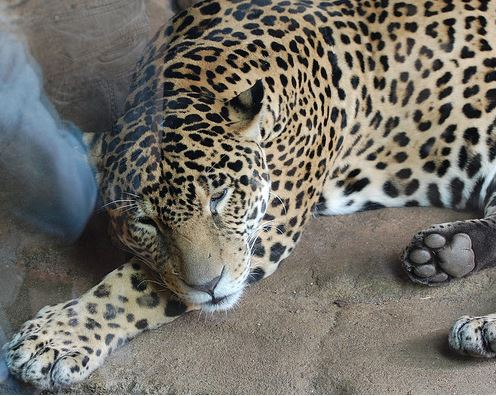
\includegraphics[width=6.0cm, trim=0 0 0 0, clip]{figures/tiger_highq.jpeg}}
		\centerline{(3a) Q=75}
%		\centerline{Baidu prediction=["leopard"]}
		\centerline{Baidu prediction \ = \ ["leopard"]}
		\vspace{0.3cm}
	\end{minipage}
	\hfill
	\begin{minipage}{0.5\linewidth}
		\centerline{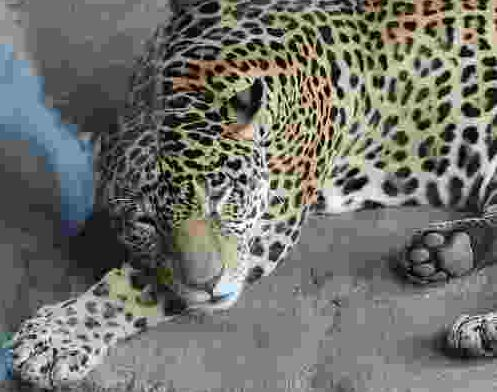
\includegraphics[width=6.0cm, trim=0 0 0 0, clip]{figures/tiger_lowq.jpeg}}
		\centerline{(3b) Q=5}
%		\centerline{Baidu prediction=["leopard"]}
		\centerline{Baidu prediction \ = \ ["leopard"]}
		\vspace{0.3cm}
	\end{minipage}
%	\end{tabular}
	\caption{The prediction of a deep learning model is not completely related to the input image's quality, making it difficult to use a fixed compression quality for all images. For image 1a, 1b and 2a, 2b, minor changes cause different predictions though they are visually similar; for image 3a and 3b, the cloud model still output correct label from a severely compressed image though they look very different}
	\label{fig: compress_accuracy}
%	\vspace{-0.1cm}
\end{figure*}

To address the above challenges, we present a reinforcement learning-based solution, called AdaCompress\footnote{We open-sourced AdaCompress that works with online computer vision-based APIs at \url{https://github.com/hosea1008/AdaCompress}}, to choose the proper compression quality level for an image to a computer vision model on the cloud, in an online manner. This paper is an extension of our earlier conference paper~\cite{2019adacompress}, with the following contributions:

$\rhd$ We design an interactive training environment that can be applied to different online computer vision-based services. We propose a Deep Q-learning Network-based~\cite{DQN} agent to evaluate and predict the performance of a compression quality level on an input image. In real-world application scenarios, this agent can be highly efficient to run on today's edge infrastructures (e.g., Google edge TPU~\cite{google-tpu}, Huawei Atlas 500 edge station~\cite{huawei-atlas500}).
	
$\rhd$ We build a reinforcement learning-based framework to train the agent in the above environment. The agent can learn to choose a proper compression quality level for an input image after iteratively interacting with the environment by feeding the carefully designed reward that considers both accuracy and data size. Based on~\cite{2019adacompress}, we further propose an \emph{explore-exploit} mechanism to let the agent switch between ``sceneries''. In particular, after deploying the agent, an \emph{inference-estimate-retrain} solution is designed to restart the training once the scenery changes and the existing running agent cannot guarantee the original accuracy performance.
	
$\rhd$~~In this journal extension, we provide more analysis and insights on our design. By analyzing the Deep Q-learning Network-based agent's behaviors using Grad-Cam~\cite{grad-cam}, we provide the reasons that the agent chooses a specific compression quality level. We reveal that images containing large smooth areas are more sensitive to compression, while images with complex textures are more robust to compression for computer vision models.
	
$\rhd$ We evaluate our system on representative cloud deep learning services, including Amazon Rekognition~\cite{amazon_rekognition}, Face++~\cite{face++_service} and Baidu Vision~\cite{baidu_vision}, and show that our design can reduce the upload traffic load by up to $1/2$ while maintaining comparable overall accuracy. Compared to baseline DeepN-JPEG~\cite{DeepN-JPEG}, the overall accuracy of AdaCompress is $8\%$ higher when they have similar compressed image size.

% \begin{itemize}
% 	\item First, we completed designing agent caching strategy work mentioned in our previous version's future work~\cite{2019adacompress}, adding the model query state in previous inference-estimate-retrain mechanism to avoid unnecessary upload traffic load in the retraining phase. Once capturing the scenery change, comparing to the previous mechanism that retrains from scratch directly, in our new mechanism, AdaCompress switches into model query state and loads a suitable RL agent model, achieving a lower upload traffic load. In the experiment, we use the FLIR Thermal Dataset instead of the previous DNIM Dataset to act as a nighttime scenery since thermal sensors capture gray-scaled thermal images in the nighttime, and the experiment result shows that our design can cut down the uploading file size overhead effectively.
% 	\item Second, for the comparison purpose, we implement the DeepN-JPEG framework according to~\cite{DeepN-JPEG} and evaluate the size reduction and accuracy performance. Our experiment shows that AdaCompress and DeepN-JPEG both decrease the uploading file size overhead more than 1/2, but the inference accuracy of AdaCompress is 8\% higher than that of DeepN-JPEG. Moreover, we provide illustrative image examples to present that AdaCompress compresses images more adaptively to achieve higher accuracy.
% 	\item Last but not least, we re-organize and amend the manuscript significantly to be easier to follow.
% \end{itemize}
The rest of this paper is organized as follows. We discuss related works in Sec.~\ref{sec: related_works}. In Sec.~\ref{sec: design} we present our framework and detailed design. We present our solution's performance in Sec.~\ref{sec: evaluation} and conclude the paper in Sec.~\ref{sec: conclusion}.

%The rest of this paper is organized as follows. We present our framework and detailed design in Sec.~\ref{sec: design}. In Sec.~\ref{sec: evaluation} we present our solution's performance. We discuss related works in Sec.~\ref{sec: related_works} and conclude the paper in Sec.~\ref{sec: conclusion}.